\documentclass[tikz]{standalone}

\newcommand{\vv}[1]{\ensuremath\textbf{#1}} % displaying vectors as bold upright quantities


\usepackage[compat=1.1.0]{tikz-feynman}
\tikzset{cross/.style={cross out, draw=black, minimum size=2*(#1-\pgflinewidth), inner sep=0pt, outer sep=0pt},
%default radius will be 1pt. 
cross/.default={1pt}}
\usepackage{amsmath}
\usepackage{euler}

\begin{document}

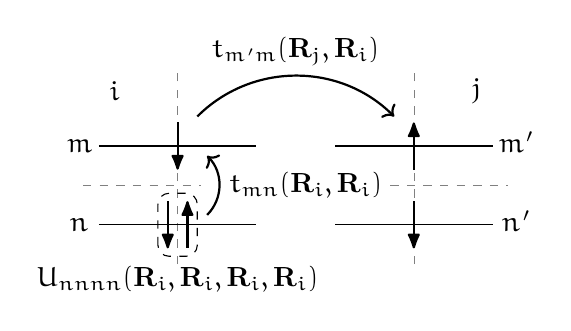
\begin{tikzpicture}
\draw[style=help lines,dashed] (1,-0.5) -- (1,2);
\draw[style=help lines,dashed] (4,-0.5) -- (4,2);
\draw[style=help lines,dashed] (-0.2,0.5) -- (1.3,0.5);
\draw[style=help lines,dashed] (3.7,0.5) -- (5.2,0.5);

% Draw orbitals (horizontal lines) for system i
\draw (0,1) -- (2,1);
\draw (0,0) -- (2,0);

% Draw orbitals (horizontal lines) for system j
\draw (3,1) -- (5,1);
\draw (3,0) -- (5,0);

% Arrows for electrons on system i
\draw[-{Latex[round]}, thick] (1,1.3) -- (1,0.7);
\draw[-{Latex[round]}, thick] (0.875,0.3) -- (0.875,-0.3);
\draw[{Latex[round]-}, thick] (1.125,0.3) -- (1.125,-0.3);

% Arrows for electrons on system j
\draw[{Latex[round]-}, thick] (4,1.3) -- (4,0.7);
\draw[-{Latex[round]}, thick] (4,0.3) -- (4,-0.3);

% Hopping terms
\draw[->, thick] (1.375,0.125) to [bend right=45] node[midway, right] {$t_{mn}(\vv{R}_i,\vv{R}_i)$} (1.375,0.875);
\draw[->, thick] (1.25,1.375) to [bend left=45] node[midway, above] {$t_{m'm}(\vv{R}_j,\vv{R}_i)$} (3.75,1.375);

% Labels for orbitals
\node at (-0.25,1) {$m$};
\node at (-0.25,0) {$n$};
\node at (5.3,1.05) {$m'$};
\node at (5.3,0.05) {$n'$};

% Labels for systems i and j
\node at (0.2,1.7) {$i$};
\node at (4.8,1.7) {$j$};

% U
\draw[dashed, rounded corners] (0.75,-0.4) rectangle (1.25,0.4);
\node at (1,-0.7) {$U_{nnnn}(\vv{R}_i,\vv{R}_i,\vv{R}_i,\vv{R}_i)$};

\end{tikzpicture}

\end{document}
